\documentclass[10pt,letterpaper, onecolumn]{article}
%\usepackage[utf8]{inputenc}
\usepackage[T1]{fontenc}    % use 8-bit T1 fonts
\usepackage{graphicx} % Required for the inclusion of images
\usepackage{epstopdf}
\usepackage{amsmath} % Required for some math elements 
\usepackage{times}
\usepackage{lipsum} % to be removed later
\usepackage{verbatim}
\usepackage{float}
\usepackage[colorlinks=true, urlcolor=blue, citecolor=blue, linkcolor =blue]{hyperref}       % hyperlinks
\usepackage{enumitem} % to remove space between enum points
% MATH PACKAGES
\usepackage{amsmath,bm}
\usepackage{amssymb}
%TABLES
\usepackage{array} % For centering the entries in a table
%FIGURES
\usepackage{subfigure}

\usepackage[title]{appendix}

% For subsubsubsection
\usepackage{titlesec}
\setcounter{secnumdepth}{4}
\titleformat{\paragraph}
{\normalfont\normalsize\bfseries}{\theparagraph}{1em}{}
\titlespacing*{\paragraph}
{0pt}{3.25ex plus 1ex minus .2ex}{1.5ex plus .2ex}

% Remove indent for all paragraphs
\usepackage{parskip} 

\usepackage{abstract}
\setlength{\absleftindent}{0mm}
\setlength{\absrightindent}{0mm}

\usepackage{xcolor}
\definecolor{shadecolor}{RGB}{230,230,230}

\usepackage{mdframed}
\mdfdefinestyle{mdfabstract}
{
    backgroundcolor=shadecolor,
    hidealllines=true,
    leftmargin=0.1\textwidth,
    rightmargin=0.1\textwidth
}

\usepackage[%showframe,
top = 1.0in, 
bottom = 1.25in,
footskip = 25pt,
marginparsep = 0pt,
headsep = 0pt]{geometry}

\title{\vspace{-3cm}
\noindent\makebox[\linewidth]{\rule{0.9\textwidth}{2.0pt}} \\ 
\textbf{Model Order Reduction using Proper Orthogonal Decomposition} \\
\vspace{-0.30cm}
\noindent\makebox[\linewidth]{\rule{0.9\textwidth}{0.5pt}}}

\author{Ramya Rao Basava\\
Department of Computer Science\\
University of British Columbia, Vancouver}

\date{}

\begin{document}

\maketitle

\textcolor{red}{\textbf{Note: This work is part of my PhD thesis at University of California San Diego and is copyrighted.}}

%========================================================
\section{Introduction}
%========================================================
The main aim of model order reduction is to find a lower dimension approximation of a full model solution by projecting it onto a lower dimensional space. Proper Orthogonal Decomposition (POD), also known as Principal Component Analysis (PCA), is one of the most popular methods used to construct this projection operator. In this method the proper orthogonal modes of a system of equations are constructed and then these modes are truncated as required to construct the lower dimensional approximation. Model reduction for the strong form Reproducing Kernel Collocation Method (RKCM) \cite{hu2011error} is proposed, where a Least Squares Galerkin projection is used to project the over-determined system of equations. Examples are provided for linear problems for the RKCM framework.

%========================================================
\section{Reduced bases from Proper Orthogonal Decomposition (POD)}
\label{section7.1}
%========================================================
In this section the detailed derivation for obtaining the reduced order POD bases is given \cite{ philipbook2012turbulence, kerschen2005method}.
Consider a function $u(\bm{x},t)$ defined on the domain $\bm{x} \in \mathbb{R}^n$, for which a approximate reduced order function is to be obtained by projection on to a reduced bases (here POD bases). The POD bases are obtained under the following statement of optimality: 

\noindent 
Find a bases $\phi$ such that; the averaged squared error between $u(\bm{x},t)$ and its orthogonal projection on to $\phi$ is minimized, \cite{philipbook2012turbulence}. This is given by the following expression:
%
\begin{equation}
\underset{\phi \in L_2}{min} \left \langle   \left \Vert    u - \frac{(u, \phi)}{\Vert \phi \Vert^2} \phi    \right \Vert^2      \right \rangle
\label{eqn7.1}
\end{equation}
%
where $(\bullet,\bullet)$ is the inner product defined by $(f,g)_{\Omega} = \int_{\Omega} f(\bm{x}) g^*(\bm{x}) d\bm{x}$. Here `$^*$' denotes the complex conjugate. $\Vert \bullet \Vert = (\bullet , \bullet)^{\frac{1}{2}}$ is the induced norm and $\langle \bullet \rangle$ is the averaging operator. This is equivalent to maximizing the averaged inner product between $u$ and $\phi$ suitably normalized \cite{ philipbook2012turbulence, kerschen2005method}:
%
\begin{equation}
\underset{\phi \in L_2}{max} \frac{ \left \langle  \vert (u,\phi) \vert^2  \right \rangle  }{\Vert \phi \Vert^2}
\label{eqn7.2}
\end{equation}
%
subject to the condition $\Vert \phi \Vert^2 = 1$. Here $\vert \bullet \vert$ denotes the absolute value. The proof for equivalence of equation \eqref{eqn7.1} and \eqref{eqn7.2} is given as follows:
%
\begin{align}
\left \langle   \left \Vert    u - \frac{(u, \phi)}{\Vert \phi \Vert^2} \phi    \right \Vert^2      \right \rangle &= 
\left \langle   \left (    u - \frac{(u, \phi)}{\Vert \phi \Vert^2} \phi  , u - \frac{(u, \phi)}{\Vert \phi \Vert^2} \phi   \right )      \right \rangle \notag \\
&= \left \langle (u,u) - 2 \frac{(u,\phi) }{\Vert \phi \Vert^2} (u,\phi) 
+   \frac{(u,\phi) }{\Vert \phi \Vert^2} \frac{(u,\phi) }{\Vert \phi \Vert^2} \Vert \phi \Vert^2   \right \rangle \notag  \\
&= \left \langle  \Vert u \Vert^2  -  \frac{\vert (u,\phi) \vert^2 }{\Vert \phi \Vert^2}  \right \rangle \notag \\
&= \left \langle  \Vert u \Vert^2 \right \rangle  - \left \langle  \frac{\vert (u,\phi) \vert^2 }{\Vert \phi \Vert^2}  \right \rangle
\end{align}
%
From the above proof, it can be seen that:
%
\begin{equation}
\underset{\phi \in L_2}{min} \left \langle   \left \Vert    u - \frac{(u, \phi)}{\Vert \phi \Vert^2} \phi    \right \Vert^2      \right \rangle
\Rightarrow \underset{\phi \in L_2}{max} \frac{ \left \langle  \vert (u,\phi) \vert^2  \right \rangle  }{\Vert \phi \Vert^2}; \quad \Vert \phi \Vert^2 = 1
\end{equation}
%

For example, consider the case when $u$ represents velocity. Equation \eqref{eqn7.2} means that if $u$ is projected along $\phi$, the average energy content (kinetic energy) is greater than if $u$ is projected along any other bases function. The maximization problem in equation \eqref{eqn7.2} can be recast into a constrained minimization problem with the functional defined by:
%
\begin{equation}
J[\phi] = \left \langle \vert (u , \phi) \vert^2 \right \rangle - \lambda \left (  \Vert \phi \Vert^2  -1 \right) 
\end{equation}
%
where $\lambda$ is the Lagrange multiplier. Using calculus of variations, the necessary condition for extrema is reached when the functional derivative vanishes for all variations of $\phi + \varepsilon \eta \in L_2$. Here $\eta \neq 0$ is an auxillary function and 
$\varepsilon \in \mathbb{R}$ is a small parameter.
%
\begin{equation}
\frac{d}{d\varepsilon} J[\phi + \varepsilon \eta] \bigg \vert_{\varepsilon = 0} = 0
\end{equation}
%
Using the inner product property; $(f,g) = (g,f)^*$, the above equation can be written as:
%
\begin{align}
&\frac{d}{d\varepsilon} \left [  \left \langle  (u , \phi + \varepsilon \eta) (\phi + \varepsilon \eta , u)   \right \rangle
- \lambda (\phi + \varepsilon \eta,\phi + \varepsilon \eta)  \right]    \bigg \vert_{\varepsilon = 0} = 0 \notag \\
\Rightarrow &2  \left [     \left \langle  (u,\eta)(\phi,u)    \right \rangle - \lambda (\phi,\eta)  \right] = 0 \notag \\
\Rightarrow &\left \langle    \int_{\Omega} u(\bm{x}) \eta^*(\bm{x}) d\bm{x}    \int_{\Omega}  \phi(\bm{x}') u^*(\bm{x}')  d\bm{x}' \right \rangle -
\lambda \int_{\Omega} \phi(\bm{x}) \eta^*(\bm{x}) d\bm{x} = 0
\end{align}
%
Interchanging the order of the averaging operator and inner product (averaging operator commutes with the integral):
%
\begin{equation}
\int_{\Omega}  \left [  \int_{\Omega}  \left \langle u(\bm{x}) u^*(\bm{x}') \right \rangle \phi(\bm{x}') d\bm{x}' - \lambda \phi(\bm{x})   \right ]  \eta^*(\bm{x}) d\bm{x}  = 0
\end{equation}
%
This results in the following Euler--Lagrange equation: 
%
\begin{equation}
\int_{\Omega}  \left \langle u(\bm{x}) u^*(\bm{x}') \right \rangle \phi(\bm{x}') d\bm{x}' = \lambda \phi(\bm{x});  \quad \forall \eta^*(\bm{x}) \neq 0
\label{eqn7.9}
\end{equation}
%
The above equation gives the integral eigenvalue problem. Here $R(\bm{x},\bm{x}') = \left \langle u(\bm{x}) u^*(\bm{x}') \right \rangle$ is the averaged auto correlation function. The solution to the integral eigenvalue problem given in equation \eqref{eqn7.9}, gives a series of eigenvector or eigenfuctions which are called Proper Orthogonal Modes ${\phi_i(x)}^{\infty}_{i=1}$ (POM's or POD modes) and the corresponding eigenvalues $\lambda^{\infty}_{i=1}$ are called Proper Orthogonal Values (POV's). The energy contained is defined as: 
%
\begin{equation}
E = \sum_{i=1}^{\infty} \lambda_i
\end{equation}
%
and the energy captured by the $i^\text{th}$ POM is given by $\lambda_i/E$. The reduced order solution to $u$ is obtained by truncating the bases and considering only the first $r$ modes which capture say around $99\%$ of energy. From the mathematical statement of optimality used for constructing the POD bases, it can be seen that on an average, the reduced POD bases form the `best' bases as the POD eigenvalues decay rapidly and capture more amount of energy in the first $r$ POD modes, than any other bases. 

Finally the approximation of $u$ denoted by $u^h$ is obtained by projecting $u$ on to the reduced POD bases as follows:
%
\begin{equation}
u(\bm{x}) \approx u^h(\bm{x}) = \sum^r_{i=1} \phi(\bm{x}) a_i  = \bm{U} \bm{a}
\end{equation}
%
where $\bm{U} = [\phi_1, \cdots, \phi_r]$ are the reduced bases functions and $\bm{a} = \{ a_1, \cdots, a_r\}$ are unknown coefficients. 


%-----------------------------------
\subsection{POD computation in the discrete case using eigenvalue analysis}
%-----------------------------------
In general the continuous governing equations are discretized in space when solving using finite difference, finite element or meshfree methods. For example consider solving a linear elastodynamics problem using the meshfree Reproducing Kernel Particle Method (RKPM), where $\bm{u}(\bm{x},t)$ is the field variable which is the displacement at point $\bm{x}$ at time $t$. The Galerkin weak form in $\bm{u}$ is discretized in space using the meshfree RK approximation to obtain the following matrix equation:
%
\begin{equation}
\bm{M} \ddot{\bm{d}} + \bm{K} \bm{d} = \bm{F}
\label{eqn7.12}
\end{equation}
%
where, $\bm{M}$ is the mass matrix of size $n \times n$ where $n$ is the number of degrees of freedom, $\bm{K}$ is the stiffness matrix of size $n \times n$, $\bm{F}$ is the force vector of size $n$ and $\bm{d}$ is the vector of nodal coordinates  of size $n$.

The method of snapshots is used to find the reduced order solution to the above equation \cite{ philipbook2012turbulence, kerschen2005method}. In the off-line phase where the full model simulations are run, a set of `$S$' snapshots of the nodal coordinate vector $\bm{d} \in \mathbb{R}^n$, at different time intervals are collected in a matrix $\bm{D}$, which is called the Response matrix and is of size $n \times S$.
% 
\begin{equation}
\bm{D} = [\bm{d}_1, \cdots, \bm{d}_S] = \begin{bmatrix} d_{11} & \cdots & d_{1S} \\
\vdots & \ddots & \vdots \\
d_{n1} & \cdots & d_{nS} \end{bmatrix}_{n \times S}
\end{equation}
%
In this chapter, when a subscript is used for matrices and vectors, this denotes their size. The discrete averaged auto-correlation matrix $\hat{\bm{R}}$ is given by:
%
\begin{equation}
\hat{\bm{R}} = \frac{1}{S} \bm{D} \bm{D}^T = \frac{1}{S} \begin{bmatrix} \sum^S_{j = 1} (d_{1j})^2 & \cdots & \sum^S_{j = 1} (d_{1j}) (d_{nj}) \\
\vdots & \ddots & \vdots \\
\sum^S_{j = 1} (d_{nj}) (d_{1j}) & \cdots &  \sum^S_{j = 1} (d_{nj})^2 \end{bmatrix}
\end{equation}
%
The eigenvalue problem in the discrete form is given by:
%
\begin{equation}
\hat{\bm{R}} \bm{U} =  \bm{U} \bm{\Lambda}
\label{eqn7.15}
\end{equation}
%
where 
\begin{equation}
\bm{U} = [\bm{\phi}_1, \cdots, \bm{\phi}_n]
\end{equation}
is the matrix containing the POD bases, and  
\begin{equation}
\bm{\Lambda} = diag(\lambda_1, \cdots, \lambda_n)
\end{equation}
is the matrix having the eigenvalues as the diagonal entries. This discrete eigenvalue problem is analogous to the continuous version given in equation \eqref{eqn7.9}. The above discrete eigenvalue problem given in equation \eqref{eqn7.15} can be solved to obtained the POD bases. In equation \eqref{eqn7.15}, the discrete averaged auto-correlation matrix $\hat{\bm{R}}$, is a self-adjoint matrix. The Hilbert-Schmidt theorem states that: `The eigenvalues of a self-adjoint matrix are real and the eigenvectors corresponding to distinct eigenvalues are orthogonal'. According to this theorem the POD bases vectors are orthogonal. 

It can be seen from \eqref{eqn7.15} that a $n \times n$ eigenvalue problem needs to be solved to obtain the POD bases, but as this part of the process can be carried out off-line, this computational expense need not be considered. In general if $n >> S$ and if it is required to reduce this off-line computational cost, the method of snapshots as proposed by Sirovich et al. in \cite{sirovich1987low} can be used. In this method the $n \times n$ eigenvalue problem is transformed to a $S \times S$ eigenvalue problem as follows. Since the POD bases and the snapshots span the same space, each eigenvector $\phi$ can be expressed as a linear combination of the snapshots. 
%
\begin{equation}
\phi = \bm{D}_{(n \times S)} \  \hat{\bm{a}}_{(S \times 1)}
\end{equation}
%
where $\hat{\bm{a}}^T = \{  \hat{a}_1, \cdots,   \hat{a}_S\}$  are the unknown coefficients. Substituting this in the discrete eigenvalue problem given in equation \eqref{eqn7.15} gives:
%
\begin{align}
&\hat{\bm{R}} \bm{U} =  \bm{U} \bm{\Lambda} \notag \\
 \Rightarrow &\frac{1}{S} \bm{D} \bm{D}^T \phi = \lambda \phi; \quad (n \times n \text{ eigenvalue problem}) \notag \\
\Rightarrow &\frac{1}{S} \bm{D} \bm{D}^T  \bm{D} \hat{\bm{a}} = \lambda \bm{D} \hat{\bm{a}} \notag \\
\Rightarrow &\frac{1}{S} \bm{D}^T  \bm{D} \hat{\bm{a}} = \lambda \hat{\bm{a}}; \quad  (S \times S \text{ eigenvalue problem})
\end{align}
%
In order for the above equation to be a necessary condition, the snapshots need to be linearly independent \cite{ philipbook2012turbulence}. Provided $\hat{\bm{a}}$ is scaled to be orthonormal, that is, $\hat{\bm{a}}^T \hat{\bm{a}} = \bm{I}$:
%
\begin{equation}
\phi^T \phi = \hat{\bm{a}}^T \bm{D}^T  \bm{D} \hat{\bm{a}} = \lambda S
\end{equation}
%
To get a set of orthonormal bases $\phi$ divide by:
%
\begin{equation}
\phi_i = \frac{1}{\sqrt{S \lambda_i}}  \bm{D} \hat{\bm{a}}_i; \quad i = 1, \cdots, S
\end{equation}
%
This results in $\phi^T \phi = \bm{I}$. In this way the first `$S$' POD modes can be obtained. 


%-----------------------------------
\subsection{POD computation in the discrete case using Singular Value Decomposition (SVD)}
%-----------------------------------

Alternately the POD bases can be equivalently obtained by SVD of the response matrix as follows:
%
\begin{equation}
\bm{D}_{(n \times S)} = \bm{U}_{(n \times n)} \   \bm{\Sigma}_{(n \times S)} \   \bm{V}^T_{(S \times S)}
\end{equation}
%
here $ \bm{U} \in \mathbb{R}^{n \times n}$ and $ \bm{V} \in \mathbb{R}^{S \times S}$ are the orthogonal matrices containing the left singular vectors and right singular vectors of $\bm{D}$, respectively. The matrix $\bm{U}$ gives the POD bases. $\bm{\Sigma} \in \mathbb{R}^{n \times S}$ is a semi positive definite psuedo-diagonal matrix and contains diagonal entries with singular values of $\bm{D}$, given by $\sigma_i$.
%
\begin{equation}
\bm{\Sigma}(i,i) = \sigma_i; \quad i = min(n,S)
\end{equation}
%
and $\sigma_1 > \sigma_2 > \cdots > \sigma_{min(n,S)} \geq 0$.

%-----------------------------------
\subsection{Equivalence of EVD and SVD}
%-----------------------------------

The equivalence between EVD and SVD and the relationship between the eigenvalues and singular values can be obtained from the following equations: 
%
\begin{align}
\frac{1}{S} \bm{D} \bm{D}^T &= \frac{1}{S} \bm{U} \bm{\Sigma} \bm{\Sigma}^T \bm{U}^T  = 
\bm{U} \ diag( \frac{\sigma_1^2}{S}, \cdots, \frac{\sigma_n^2}{S} ) \ \bm{U}^T \\
\frac{1}{S}  \bm{D}^T \bm{D} &= \frac{1}{S} \bm{V} \bm{\Sigma}^T \bm{\Sigma} \bm{V}^T = 
\bm{V} \ diag( \frac{\sigma_1^2}{S}, \cdots, \frac{\sigma_S^2}{S} )  \ \bm{V}^T
\end{align}
%
From the above equations, the relationship between the eigenvalues and singular values is given by:
%
\begin{equation}
\lambda_i = \frac{\sigma^2_i}{S}
\end{equation}
%



%========================================================
\section{Galerkin and Petrov-Galerkin projections}
%========================================================

Consider the general case of the matrix equation for a linear elastodynamics problem as given in equation \eqref{eqn7.12}. The reduced order approximation for $\bm{d}$ denoted by $\bm{d}^h$ is given by the expression: 
%
\begin{equation}
\bm{d}^h_{(n \times 1)} = \bar{\bm{U}}_{(n \times r)} \  \bm{d}^r_{(r \times 1)}
\label{eqn7.27}
\end{equation}
%
where $r$ is the order of reduction with $r << n$, $\bar{\bm{U}} = [\phi_1, \cdots, \phi_r]$ is the projection matrix containing the reduced set of POD bases and $ \bm{d}^r$ are the reduced nodal coordinates. Substituting equation \eqref{eqn7.27} in the system of equations \eqref{eqn7.12} gives:
%
\begin{equation}
\bm{M} \bar{\bm{U}} \ddot{\bm{d}^r} + \bm{K} \bar{\bm{U}}  \bm{d}^r - \bm{F} = \bm{e}
\end{equation}
% 
where `$\bm{e}$' is the residual error as the approximation of $\bm{d}$ is substituted in the matrix equations \eqref{eqn7.12}. In order to minimize this error, the residual error is constrained to be orthogonal to a subspace $\mathbb{W}$, defined by the bases $\bm{W} \in \mathbb{R}^{n \times r}$, which gives:
%
\begin{align}
&\bm{W}^T \bm{e} = \bm{0} \notag \\
&\bm{W}^T\bm{M} \bar{\bm{U}} \ddot{\bm{d}^r} + \bm{W}^T\bm{K} \bar{\bm{U}}  \bm{d}^r - \bm{W}^T\bm{F} = \bm{0}
\end{align}
%
For the case of Galerkin projection, $\bm{W} = \bm{\bar{U}}$ and in the case of a Petrov-Galerkin projection, $\bm{W} \neq \bm{\bar{U}}$. 

Finally the reduced system of equations are given by:
%
\begin{equation}
\hat{\bm{M}} \ddot{\bm{d}^r} + \hat{\bm{K}} \bm{d^r} = \hat{\bm{F}}
\label{eqn7.30}
\end{equation}
%
where 
%
\begin{subequations}
\begin{align}
\hat{\bm{M}}_{(r \times r)} &= \bm{W}^T_{(r \times n)} \ \bm{M}_{(n \times n)} \  \bar{\bm{U}}_{(n \times r)} \\
\hat{\bm{K}}_{(r \times r)} &= \bm{W}^T_{(r \times n)} \ \bm{K}_{(n \times n)} \  \bar{\bm{U}}_{(n \times r)} \\
\hat{\bm{F}}_{(r \times 1)} &= \bm{W}^T_{(r \times n)} \ \bm{F}_{(n \times 1)}
\end{align}
\end{subequations}
%
The matrices $\hat{\bm{M}}_{(r \times r)}$ and $\hat{\bm{K}}_{(r \times r)}$ are usually fully populated. POD transforms large sparse matrices to small dense systems. Equation \eqref{eqn7.30} gives the reduced system with $r$ degrees of freedom and can be solved for $\bm{d^r}$. The reduced solution $\bm{d}^h$ can be obtained from equation \eqref{eqn7.27}. It can be seen that when $r << n$, the computational cost for solving the system is greatly reduced. For discrete systems, the number of POD modes to be considered for the reduced system can be chosen such that the energy given by:
%
\begin{equation}
E = \frac{\sum^r_{i=1}\lambda_i}{\sum^n_{i=1}\lambda_i}
\end{equation}
%
is greater close to 1. The critical part in model order reduction using POD is choosing the correct snapshots which capture the response of the full model which is essential to give results close to the full scale model.

%========================================================
\section{Model order reduction using least squares Galerkin projection for RKCM}
%========================================================

In meshfree RKCM \cite{hu2011error}, the formulation results in solving an over-determined system of equations. This over-determined system of equations cannot be projected using a standard Galerkin projection, as this projection is not compatible. To overcome this, the Least Squares Galerkin (LSG) projection is proposed to be used in conjunction with RKCM to form the reduced set of equations in the RKCM framework. Using the LSG projection the bases $\bm{W}$ is chosen to be $\bm{K}_{(n \times n)} \  \bar{\bm{U}}_{(n \times r)}$. This method is detailed in the following section with linear problems as examples and error estimates are given to demonstrate the effectiveness of the method.

%--------------------------------------------
\subsection{Linear problems - Elastodynamics}
\label{section7.3.1}
%--------------------------------------------

Consider the following general linear elastodynamics problem for RKCM.
%
\begin{equation}
\alpha \ddot{\bm{u}}(\bm{x},t) + \bm{L}\bm{u}(\bm{x},t)  = \bm{f}(\bm{x},t) ; \quad \bm{x} \in \Omega, \ t \in (0,T]
\end{equation}
%
with boundary conditions,
%
\begin{subequations}
\begin{align}
\bm{B}^h\bm{u}(\bm{x},t)  = \bm{h}(\bm{x},t) ; \quad \bm{x} \in \partial \Omega^h, \ t \in (0,T] \\
\bm{B}^g\bm{u}(\bm{x},t)  = \bar{\bm{u}}(\bm{x},t); \quad \bm{x} \in \partial \Omega^g, \ t \in (0,T] 
\end{align}
\end{subequations}
%
and initial conditions
%
\begin{subequations}
\begin{align}
\bm{u}(\bm{x},0) = \bm{u}^0(\bm{x}); \quad \bm{x} \in \bar{\Omega} \\
\bm{\dot{u}}(\bm{x},0) = \bm{v}^0(\bm{x}); \quad \bm{x} \in \bar{\Omega}
\end{align}
\end{subequations}
%
where $\bm{L}$, $\bm{B}^h$ and $\bm{B}^g$ are the spacial differential operators in the domain, on the natural and essential boundary, respectively. $\bm{u}$ is the displacement vector, $\bm{f}$, $\bm{h}$ and $\bar{\bm{u}}$ are the body force, applied boundary traction vector and prescribed displacement vector, respectively. $\alpha$ is the density. $\bm{u}^0$ is the initial displacement vector, $\bm{v}^0$ is the initial velocity vector and $\bar{\Omega} = \Omega \cup \partial \Omega^h \cup \partial \Omega^g$ represents the entire problem domain. 

The temporal discretization is carried out using the central difference scheme as follows:
%
\begin{subequations}
\begin{align}
&\alpha ( \bm{u}_{n+1}(\bm{x}) -2\bm{u}_{n}(\bm{x}) + \bm{u}_{n-1}(\bm{x}) ) +
\Delta t^2 \bm{L} \bm{u}_{n}(\bm{x}) = 
\Delta t^2 \underbrace{\bm{f}(\bm{x},t_n)}_{\bm{f}_n(\bm{x})}; \quad \bm{x} \in \Omega \\
& \bm{B}^h \bm{u}_{n+1}(\bm{x}) = \underbrace{\bm{h} (\bm{x},t_{n+1})}_{\bm{h}_{n+1}(\bm{x})} ; \quad \bm{x} \in \partial \Omega^h \\
& \bm{B}^g \bm{u}_{n+1}(\bm{x}) = \underbrace{\bar{\bm{u}} (\bm{x},t_{n+1})}_{\bar{\bm{u}}_{n+1}(\bm{x})} ; \quad \bm{x} \in \partial \Omega^g \\
&\bm{u}_0 (\bm{x}) = \bm{u}^0(\bm{x}); \quad \bm{x} \in \bar{\Omega} \\
&\bm{u}_1 (\bm{x}) - \bm{u}_0 (\bm{x}) = \Delta t \bm{v}^0(\bm{x}); \quad \bm{x} \in \bar{\Omega}
\end{align}
\label{eqn7.36}
\end{subequations}
%
Here $n$ is the time step counter and $\bm{u}_n(x) = \bm{u}(\bm{x},t_n)$. For the spatial discretization, $\bm{u}_n(\bm{x})$ is discretized using the Reproducing Kernel (RK) shape function as follows:
%
\begin{equation}
\bm{u}_n(\bm{x}) \approx \bm{u}^h_n(\bm{x})=\bm{\Psi}^T (\bm{x}) \bm{a}_n
\label{eqn7.37}
\end{equation}
%
where $\bm{\Psi}^T = \left[ \bm{\Psi}_1, \bm{\Psi}_2, \cdots, \bm{\Psi}_{N_S} \right]$ with $\bm{\Psi}_I = \Psi_I \bm{I}_{\hat{d} \times \hat{d}}$ and 

\noindent
$\bm{a}^T_n = \left\{ (\bm{a}_1^T)_n, (\bm{a}_2^T)_n, \cdots, (\bm{a}_{N_S}^T)_n \right\}$ with $(\bm{a}_I^T)_n=\left\{ (a_{1I})_n, (a_{2I})_n, \cdots, (a_{\hat{d}I})_n \right\}$. Here $\Psi_I$ represents the RK shape function at node `$I$'. The discretization points for constructing the approximation of $\bm{u}_n$ are the source points $N_S$. $\bm{I}_{\hat{d} \times \hat{d}}$ is the identity matrix of size $\hat{d} \times \hat{d}$ where $\bm{u}_n \in \mathbb{R}^{\hat{d}}$. Consider a set of collocation points in the entire domain including the boundaries, with $N_P$ points in the interior of domain, $N_Q$ points on the natural boundary and $N_R$ points on the essential boundary. The approximation of $\bm{u}_n$ given in equation \eqref{eqn7.37} is substituted in the strong form of the governing equations \eqref{eqn7.36} and the residual is enforced to be zero at the collocation points which leads to an over-determined system of equations given by: 
%
\begin{subequations}
\begin{align}
&\bm{M} \bm{a}_{n+1} = \underbrace{2\bm{M} \bm{a}_{n} - \bm{M} \bm{a}_{n-1} - \Delta t^2 \bm{A}^1 \bm{a}_n + \Delta t^2 \bm{F}_n }_{\bm{b}^1_{n,n-1}} \\
& \bm{A}^2 \bm{a}_{n+1} = \bm{b}^2_{n+1} \\
&\bm{A}^3 \bm{a}_{n+1} = \bm{b}^3_{n+1}
\end{align}
\label{eqn.7.38dd}
\end{subequations}
%
where
%
\begin{subequations}
\begin{align}
&\bm{M} = \begin{bmatrix} \alpha \bm{\Psi}(\bm{p}_1) \\ \vdots \\ \alpha \bm{\Psi}(\bm{p}_{N_P}) \end{bmatrix}; \quad
\bm{A}^1 =  \begin{bmatrix}  \bm{L}\bm{\Psi}(\bm{p}_1)  \\ \vdots \\ \bm{L}\bm{\Psi}(\bm{p}_{N_P})
\end{bmatrix}; \quad
\bm{F}_n(t) = \begin{bmatrix} \bm{f}(\bm{p}_1,t_n)  \\ \vdots \\  \bm{f}(\bm{p}_{N_P},t_n) \end{bmatrix} \\
&\bm{A}^2 = \begin{bmatrix}   \bm{B}^h  \bm{\Psi}(\bm{q}_1) \\ \vdots \\ 
 \bm{B}^h  \bm{\Psi}(\bm{q}_{N_Q}) \end{bmatrix}; \quad
\bm{b}^2_{n+1} = \begin{bmatrix}   \bm{h}(\bm{q}_1,t_{n+1})  \\ \vdots \\ 
 \bm{h}(\bm{q}_{N_Q},t_{n+1}) \end{bmatrix} \\
& \bm{A}^3 = \begin{bmatrix}   \bm{B}^g  \bm{\Psi}(\bm{r}_1) \\ \vdots \\  
 \bm{B}^g  \bm{\Psi}(\bm{r}_{N_R}) \end{bmatrix}; \quad
\bm{b}^3_{n+1} = \begin{bmatrix}   \bm{g}(\bm{r}_1,t_{n+1})  \\ \vdots \\ 
 \bm{g}(\bm{r}_{N_R},t_{n+1}) \end{bmatrix}
\end{align}
\end{subequations}
%
Re-writing equations \eqref{eqn.7.38dd} with added weights on the essential and natural boundaries:
%
\begin{equation}
\underbrace{\begin{bmatrix} \bm{M} \\ \sqrt{\beta^h} \bm{A}^2 \\ \sqrt{\beta^g}\bm{A}^3 \end{bmatrix} }_{\bm{A}}
\bm{a}_{n+1}
= \underbrace{ \begin{bmatrix}  \bm{b}^1_{n,n-1} \\ \sqrt{\beta^h} \bm{b}^2_{n+1} \\ \sqrt{\beta^g} \bm{b}^3_{n+1} \end{bmatrix}}_{\bm{b}}
\label{eqn7.40}
\end{equation}
%
here, $\sqrt{\beta^h}$ and $\sqrt{\beta^g}$ are the weights to be applied on the natural and essential boundaries, respectively, to balance the error between the domain and the boundary terms. They are given by \cite{chi2013dispersion}: 
%
\begin{subequations}
\begin{align}
\sqrt{\beta^h} &=  \mathcal{O}(\kappa^{-1} N_S^{-2} \sigma) \\
\sqrt{\beta^g} &=  \mathcal{O}(N_S^{-1} \sigma)
\end{align}
\end{subequations}
%
where $\kappa$ is the material constant and $ \sigma  = max(\alpha, \Delta t^2, N_S^2)$. The initial conditions are given by:
%
\begin{subequations}
\begin{align}
\bm{H} \bm{a}_0 &= \bar{\bm{u}}_0 \\
\bm{H} (\bm{a}_1 - \bm{a}_0) &= \Delta t  \bar{\bm{v}}_0 \Rightarrow \bm{H} \bm{a}_1 =  \Delta t \bar{\bm{v}} + \bm{H} \bm{a}_0
\end{align}
\end{subequations}
%
where the matrices are given by:
%
\begin{equation}
\bm{H} = \begin{bmatrix}   \bm{\Psi}^T(\bm{\chi}_1)  \\ \vdots \\  \bm{\Psi}^T(\bm{\chi}_{N_C})  \end{bmatrix}; \quad 
\bar{\bm{u}}_0 = \begin{bmatrix}  \bm{u}_0(\bm{\chi}_1) \\ \vdots \\  \bm{u}_0(\bm{\chi}_{N_C}) \end{bmatrix}; \quad
\bar{\bm{v}}_0 = \begin{bmatrix}   \bm{v}_0(\bm{\chi}_1) \\ \vdots \\  \bm{v}_0(\bm{\chi}_{N_C})   \end{bmatrix}
\end{equation}
%
where $\bm{\chi} = [\bm{\chi}_1, \cdots, \bm{\chi}_{N_C}] =  \left[ \bm{p}_1, \cdots, \bm{p}_{N_P}, \bm{q}_1, \cdots, \bm{q}_{N_Q}, \bm{r}_1, \cdots, \bm{r}_{N_R} \right]$ are the collocation points and $N_C = N_P + N_Q + N_R$. The over-determined system of equations \eqref{eqn7.40} can be solved using the method of least squares. 

%--------------------------------------------
\subsubsection{Model order reduction using Least Squares Galerkin projection:}
%--------------------------------------------

The over-determined system of equations $\bm{A} \bm{a}_{n+1} = \bm{b}$ are reduced as follows. Consider a one-dimensional case where the over-determined system matrices have the following size:
%
\begin{equation}
\bm{A}_{(N_C \times N_S)} \ (\bm{a}_{n+1})_{(N_S,1)} = (\bm{b})_{(N_C,1)}
\label{eqn7.44}
\end{equation}
%
 The reduced approximation of $\bm{a}$ is given by:
%
\begin{equation}
\bm{a} \approx \bm{a}^h_{(N_S \times 1)}  = \bar{\bm{U}}_{(N_S \times r)}  \bm{a}^r_{(r \times 1)}
\label{eqn7.45}
\end{equation}
%
where $\bar{\bm{U}} = [\phi_1, \cdots, \phi_r]$ is the reduced bases obtained by truncating POD modes of the response matrix and $r$ is the number of reduced modes or the reduced degrees of freedom for solving the reduced system. $ \bm{a}^r$ are the unknown coefficients in the reduced system. Substituting the reduced approximation \eqref{eqn7.45} in \eqref{eqn7.44} results in the equation: 
%
\begin{equation}
\bm{A}_{(N_C \times N_S)} \ \bar{\bm{U}}_{(N_S \times r)}  \bm{a}^r_{(r \times 1)} - (\bm{b})_{(N_C,1)} = \bm{e}
\end{equation}
%
where $\bm{e}$ is the residual error. To minimize this error, the residual error is constrained to be orthogonal to a subspace $\mathbb{W}$, defined by the bases $\bm{W} \in \mathbb{R}^{N_C \times r}$, which gives:
%
\begin{align}
&\bm{W}^T \bm{e} = \bm{0} \notag \\
\Rightarrow &\bm{W}^T_{(r \times N_C)} \bm{A}_{(N_C \times N_S)} \ \bar{\bm{U}}_{(N_S \times r)}  \bm{a}^r_{(r \times 1)} = \bm{W}^T_{(r \times N_C)} (\bm{b})_{(N_C,1)} 
\end{align}
%
It can be seen that the bases $\bm{W}$ should belong to $\mathbb{R}^{N_C \times r}$ for projecting the RKCM equations. A projection using $\bm{W} = \bm{\bar{U}}$ is not possible since in this case $\bm{W} \in \mathbb{R}^{N_S \times r}$. Hence a Least Squares Galerkin projection is used with: 
%
\begin{equation}
\bm{W} = \bm{A}_{(N_C \times N_S)} \ \bar{\bm{U}}_{(N_S \times r)}
\end{equation}
% 
This results in the reduced equation:
%
\begin{equation}
(\bm{A}_{(N_C \times N_S)} \ \bar{\bm{U}}_{(N_S \times r)})^T \bm{A}_{(N_C \times N_S)} \ \bar{\bm{U}}_{(N_S \times r)}  \bm{a}^r_{(r \times 1)} = (\bm{A}_{(N_C \times N_S)} \ \bar{\bm{U}}_{(N_S \times r)})^T (\bm{b})_{(N_C,1)} 
\end{equation}
%
which is re-written as:
%
\begin{equation}
\bar{\bm{U}}^T_{(r \times N_S)} \bm{A}^T_{(N_S \times N_C)} 
\bm{A}_{(N_C \times N_S)} \ \bar{\bm{U}}_{(N_S \times r)}  \bm{a}^r_{(r \times 1)} 
=  \bar{\bm{U}}^T_{(r \times N_S)} \bm{A}^T_{(N_S \times N_C)}  (\bm{b})_{(N_C,1)} 
\label{eqn7.50}
\end{equation}
%
As the above system of equations \eqref{eqn7.50} has a symmetric matrix $\bar{\bm{U}}^T \bm{A}^T 
\bm{A} \ \bar{\bm{U}}$ on the left hand side, Cholesky decomposition can be used to solve these reduced determined system of equations.

%--------------------------------------------
\subsubsection{Error analysis for linear dynamic problems}
%--------------------------------------------

The error between the full and reduced solution is determined using the following error estimate: 
%
\begin{equation}
e_1 = \sum^n_{t_s = 1} \left (  \frac{||| \bm{u}_{\text{full}} - \bm{u}_{\text{red}} |||}
{||| \bm{u}_{\text{full}} |||} \right )
\end{equation}
% 
where $t_s$ denotes the time step counter and $n$ is the total number of time steps, $\bm{u}_{\text{full}}$ is the full scale solution evaluated at a set of $\hat{N}$ points in the problem domain and obtained off-line, $\bm{u}_{\text{red}}$ is the reduced order solution evaluated at the same set of $\hat{N}$ points. The norm $||| \bullet |||$ is defined as follows:
%
\begin{equation}
||| \bm{x} ||| = \frac{\sqrt{\sum^{\hat{N}}_{i = 1}  (x_i)^2  } }{\sqrt{\hat{N}}}
\end{equation}
%
where $\hat{N}$ is the length of the vector $\bm{x}$.

%--------------------------------------------
\subsubsection{Numerical examples}
%--------------------------------------------
%\vspace{0.25cm}
\noindent \textbf{Example 1: 1D Wave equation}
%--------------------------------------------

Consider a 1D string clamped at both ends. The governing equation of motion is given by:
%
\begin{equation}
\alpha \ddot{u} = E u_{,xx}; \quad x \in [0, L], \ t \in [0, T]
\end{equation}
%
with boundary conditions: 
%
\begin{subequations}
\begin{align}
& u(0,t) = 0 \\
& u(L,t) = 0
\end{align}
\end{subequations}
%
and with initial conditions:
%
\begin{subequations}
\begin{align}
& u(x,0) = 0 \\
& \dot{u}(x,0) = \omega sin(kx)
\end{align}
\end{subequations}
%
The following values for the parameters are used: density $\alpha = 1$, length $L=16$, Young's modulus $E=1$, wavenumber $k = 5 \pi /L$ and the total time $T = 6$. The angular frequency is given by $\omega = k c$, where $c = \sqrt(E/\alpha)$. A time step of $\Delta t = 0.2$ is used. For RKCM the domain is discretized using $N_S = 51$ and $N_C = 2 N_S-1$ collocation points. A support size of $3h$ is used in the RK approximation function where $h$ is the nodal spacing of the source points. A total of $31$ snapshots are collected. The decay of the first $31$ POV's is shown in figure \ref{fig:7.1}. As the eigenvalues decay very rapidly after the first eigenvalue, for the reduced order solution the number of POD modes is chosen to be $r=1$ which is $1.96\%$ of degrees of freedom (DOF) of the full model. Figure \ref{fig:7.2} shows the comparison of the full solution for $u$ and the reduced solution for $u$ at the mid point of the domain at each time step. Figure \ref{fig:7.3} shows the comparison of the full solution and the reduced solution at all the points in the domain at the final time $T = 6$. It can be seen that the reduced solution is very close to the full order solution. Table \ref{table:7.1} gives the error $e_1$ for different values of $r$. It can be seen that the error reduces as the number of modes $r$ are increased, as expected.
%
%
\begin{figure}[H]  % [t] - top, b - bottom, h - here
  \begin{center}
    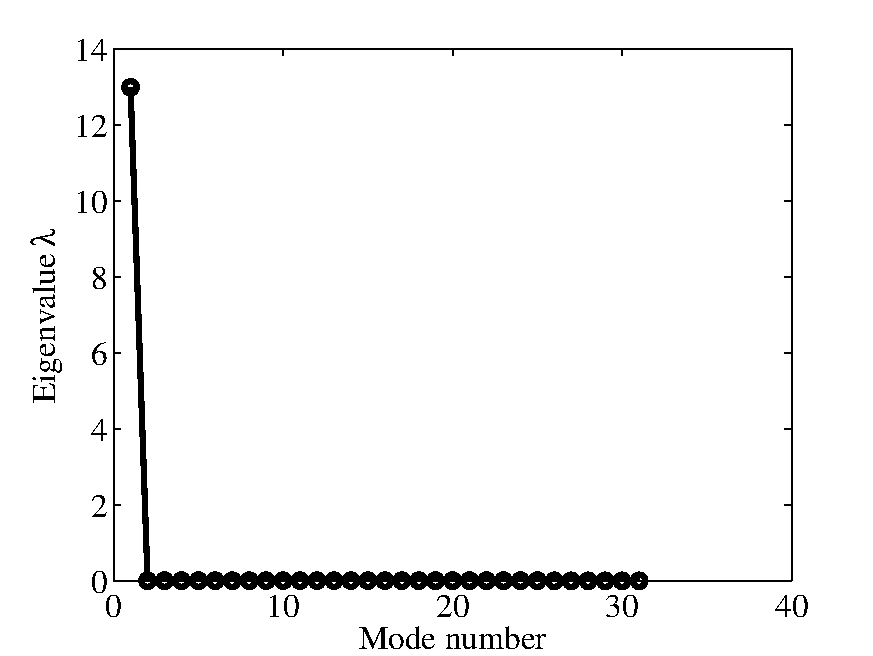
\includegraphics[width=0.42\textwidth,keepaspectratio=1,scale=1]{images/string_decay-eps-converted-to.pdf}
  \end{center}
  \caption{Decay of Proper Orthogonal Values for the 1D wave equation problem}
  \label{fig:7.1}
\end{figure}
%
%
\begin{figure}[H]  % [t] - top, b - bottom, h - here
  \begin{center}
    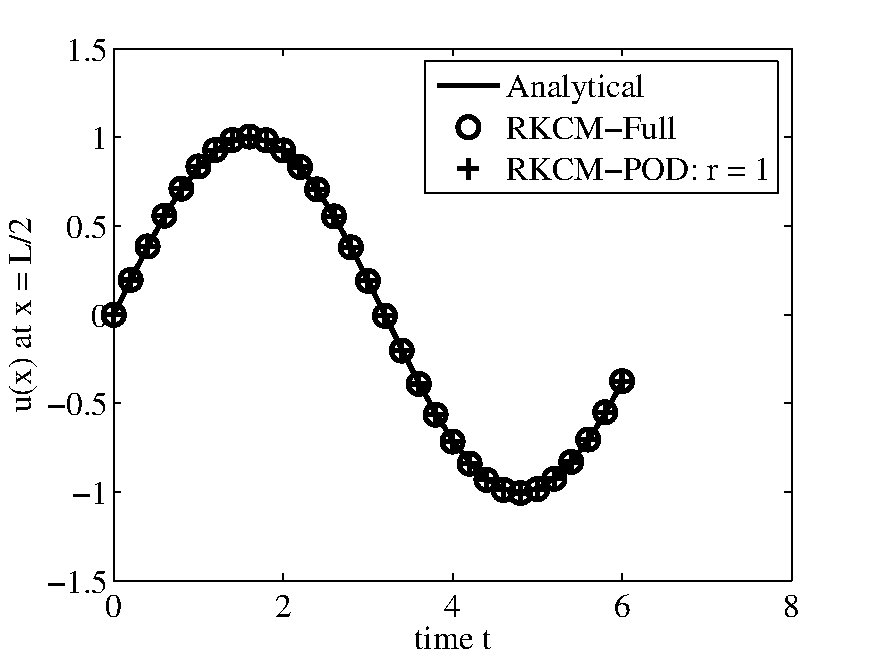
\includegraphics[width=0.5\textwidth,keepaspectratio=1,scale=1]{images/string_mid-eps-converted-to.pdf}
  \end{center}
  \caption{Comparison of the solution at the mid point of the domain, plotted for $t \in [0,T]$ for 1D wave equation problem}
  \label{fig:7.2}
\end{figure}
%
%
\begin{figure}[H]  % [t] - top, b - bottom, h - here
  \begin{center}
    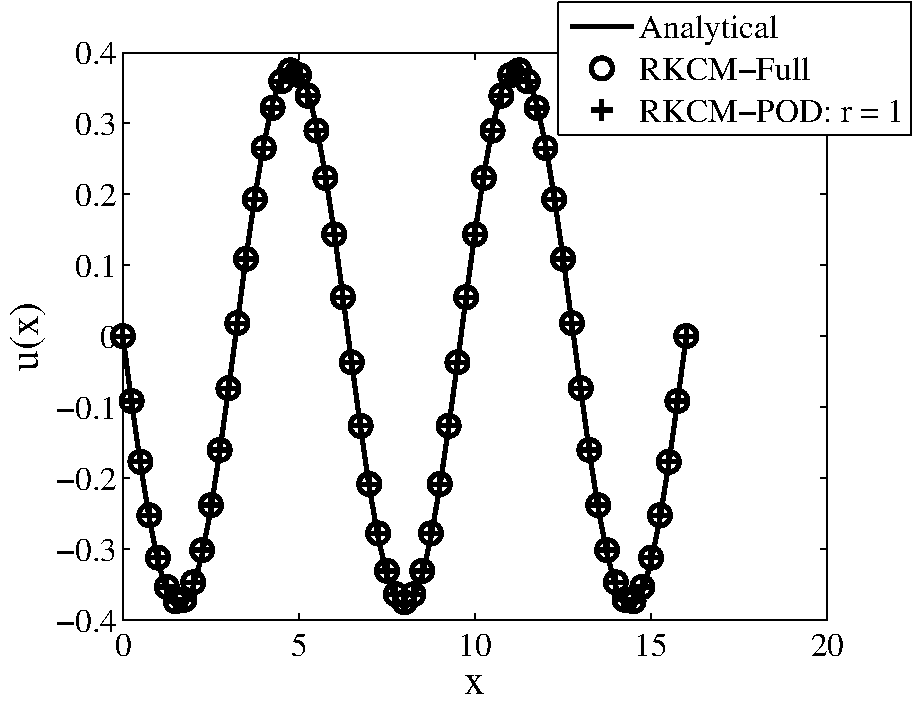
\includegraphics[width=0.5\textwidth,keepaspectratio=1,scale=1]{images/string_T-eps-converted-to.pdf}
  \end{center}
  \caption{Comparison of the solution at the final time $T=6$ plotted over the domain, for 1D wave equation problem}
  \label{fig:7.3}
\end{figure}
%
%
\begin{table}[H] 
\caption{Error $e_1$ for 1D wave equation problem}
\label{table:7.1}
\begin{center}
\begin{tabular}{| >{\centering\arraybackslash} m{2cm}| >{\centering\arraybackslash} m{2.5cm} | >{\centering\arraybackslash} m{2.5cm} |} 
\hline 
$r$ & \% DOF of full model & $e_1$  \\ %[0.5ex] % Vertical spacing
\hline \hline 
1 & 1.96\% & 3.202E-003  \\ 
\hline  
5 & 9.8\% & 4.791E-004  \\ 
\hline  
25 & 49.02\% & 5.597E-009  \\ 
\hline  
\end{tabular}
\end{center}
\end{table}
%
%

%--------------------------------------------
%\vspace{0.25cm}
\noindent \textbf{Example 2: 1D Bar with heterogeneous material}
%--------------------------------------------

Consider a 1D heterogeneous bar clamped at both ends as shown figure \ref{fig:7.4}.
%
%
\begin{figure}[H]  % [t] - top, b - bottom, h - here
  \begin{center}
    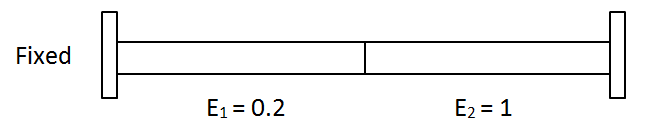
\includegraphics[width=0.5\textwidth,keepaspectratio=1,scale=1]{images/Bimaterial_bar.png}
  \end{center}
  \caption{1D bimaterial bar with clamped ends}
  \label{fig:7.4}
\end{figure}
%
%
The governing equation of motion is given by:
%
\begin{equation}
\alpha \ddot{u} = (E(x) u_{,x})_{,x}; \quad x \in [0, L], \ t \in [0, T]
\end{equation}
%
with boundary conditions: 
%
\begin{subequations}
\begin{align}
& u(0,t) = 0 \\
& u(L,t) = 0
\end{align}
\end{subequations}
%
and with initial conditions:
%
\begin{subequations}
\begin{align}
& u(x,0) = 0 \\
& \dot{u}(x,0) = sin(kx)
\end{align}
\end{subequations}
%
% 
A smooth transition of material properties at the interface is considered where the 

\noindent Young's modulus is interpolated using the RK approximation functions with linear bases and a support size of $4h$. The interpolated $E$ values and $E_{,x}$ values plotted over the domain are shown in figure \ref{fig:7.5}. 
%
%
\begin{figure}[H] % t - top, b - bottom, h - here
  \begin{center}
    \subfigure[Interpolation of $E$]{\label{fig:7.5a}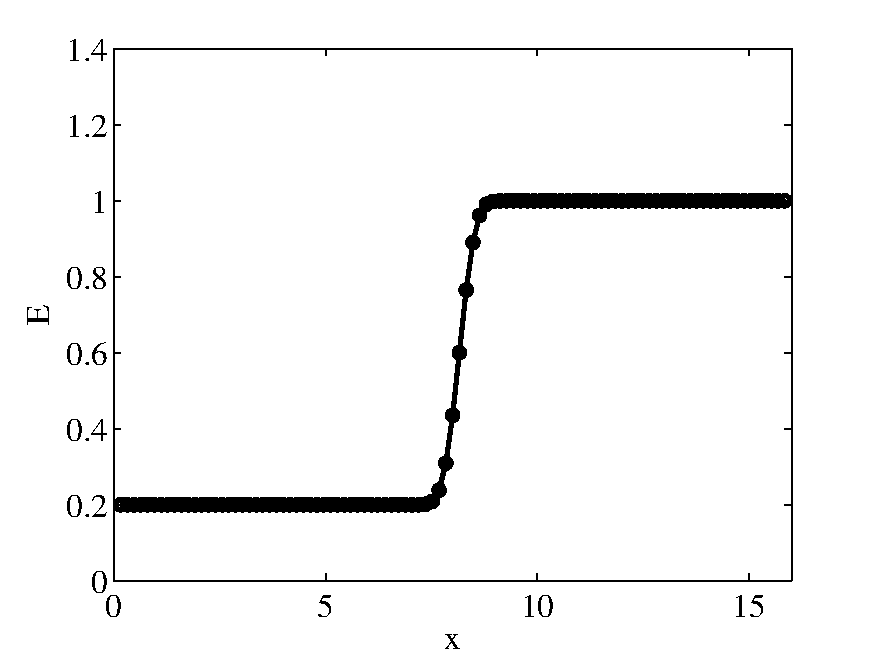
\includegraphics[width=0.495\textwidth,keepaspectratio=1,scale=1]{images/E-eps-converted-to.pdf}} \hfill % default file extension is .eps
% \hfill aligns the figures to page margins of the left and right with space in between the figures
    \subfigure[Interpolation of $E_{,x}$]{\label{fig:7.5b}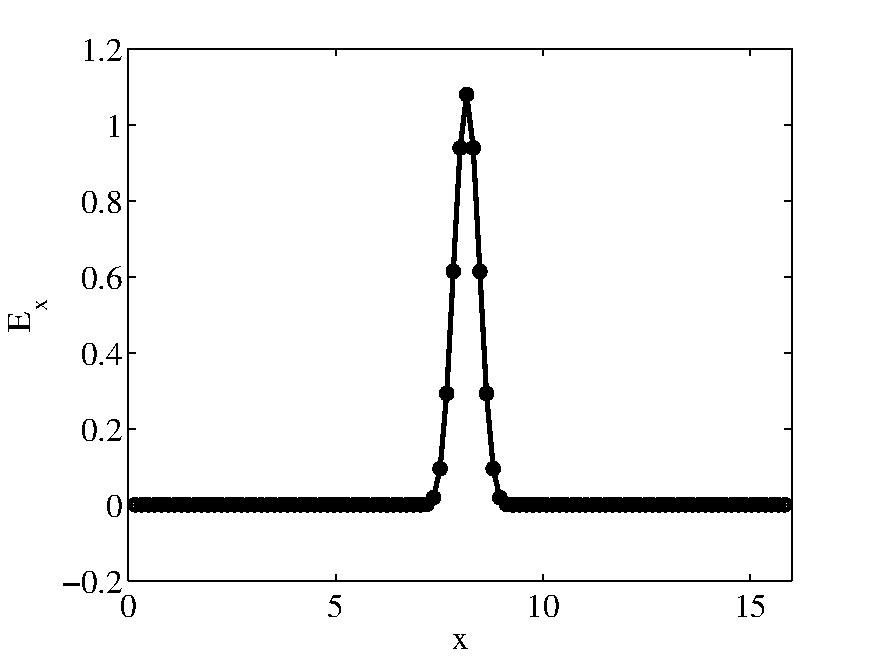
\includegraphics[width=0.495\textwidth,keepaspectratio=1,scale=1]{images/Ex-eps-converted-to.pdf}} \hfill
  \end{center}
  \caption{Interpolation of $E$ and $E_{,x}$ in the domain using RK approximation function}
  \label{fig:7.5}
\end{figure}
%
%
The following values for the parameters are used: density $\alpha = 1$, length $L=16$, wavenumber $k = 2 \pi /L$ and the total time $T = 6$.  A time step of $\Delta t = 0.2$ is used. For RKCM the domain is discretized using $N_S = 51$ and $N_C = 2 N_S-1$ collocation points. A support size of $3h$ is used in the RK approximation function where $h$ is the nodal spacing of the source points. A total of $31$ snapshots are collected. The decay of the first $31$ POV's is shown in figure \ref{fig:7.6}. Considering the eigenvalues decay, for the reduced order solution the number of POD modes is chosen to be $r=5$ which is $9.8\%$ of degrees of freedom (DOF) of the full model. Figure \ref{fig:7.7} shows the comparison of the full solution for $u$ and the reduced solution for $u$ at the mid point of the domain at each time step. Figure \ref{fig:7.8} shows the comparison of the full solution and the reduced solution at all the points in the domain at the final time $T = 6$. It can be seen that the reduced solution is very close to the full order solution. Table \ref{table:7.2} gives the error $e_1$ for different values of $r$. It can be seen that the error reduces as the number of modes $r$ are increased, as expected.
%
%
\begin{figure}[H]  % [t] - top, b - bottom, h - here
  \begin{center}
    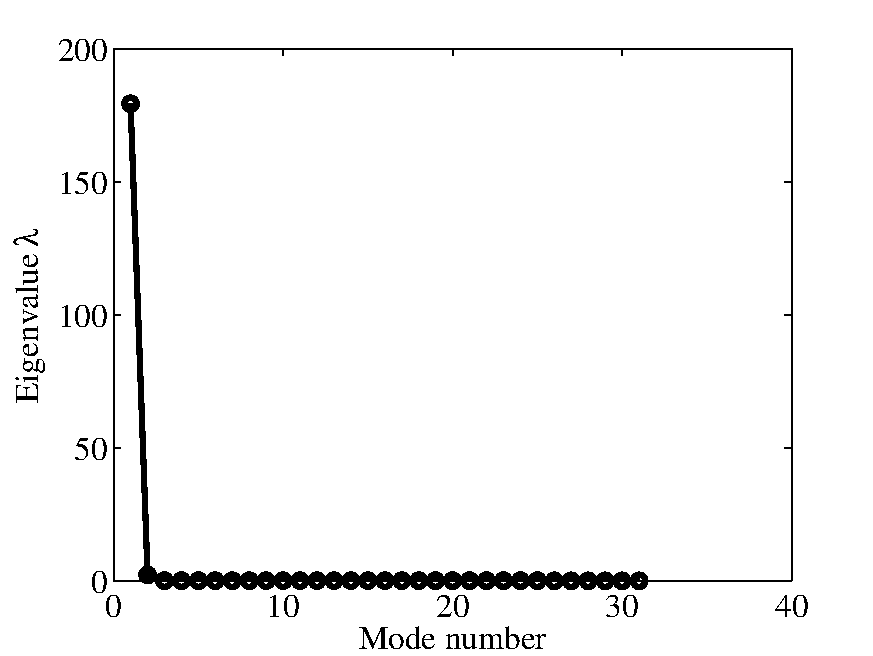
\includegraphics[width=0.45\textwidth,keepaspectratio=1,scale=1]{images/EV_bibar-eps-converted-to.pdf}
  \end{center}
  \caption{Decay of Proper Orthogonal Values for the 1D heterogeneous bar problem}
  \label{fig:7.6}
\end{figure}
%
%
\begin{figure}[H] % [t] - top, b - bottom, h - here
  \begin{center}
    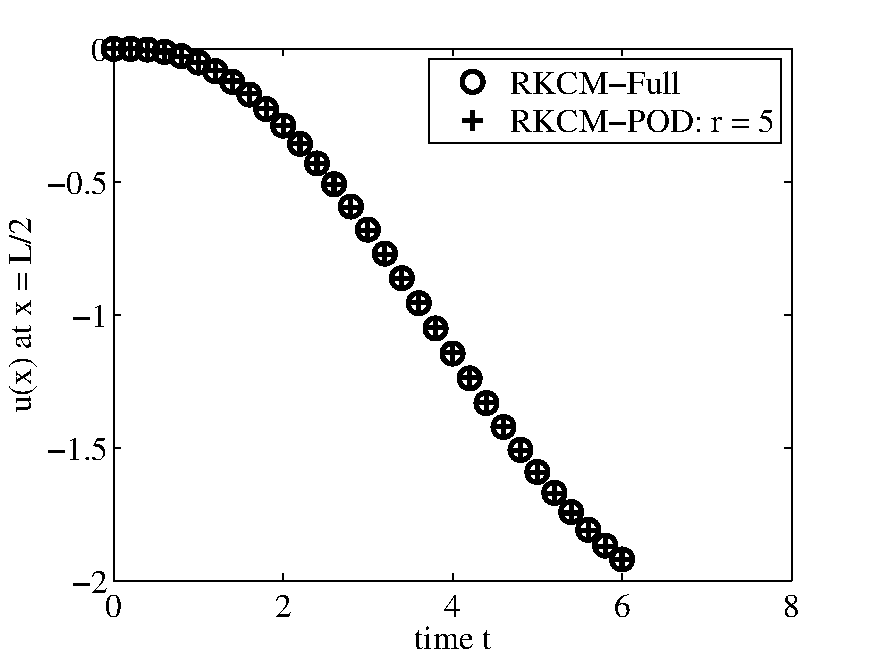
\includegraphics[width=0.5\textwidth,keepaspectratio=1,scale=1]{images/bar_mid-eps-converted-to.pdf}
  \end{center}
  \caption{Comparison of the solution at the mid point of the domain, plotted for $t \in [0,T]$ for 1D heterogeneous bar problem}
  \label{fig:7.7}
\end{figure}
%
%
\begin{figure}[H] % [t] - top, b - bottom, h - here
  \begin{center}
    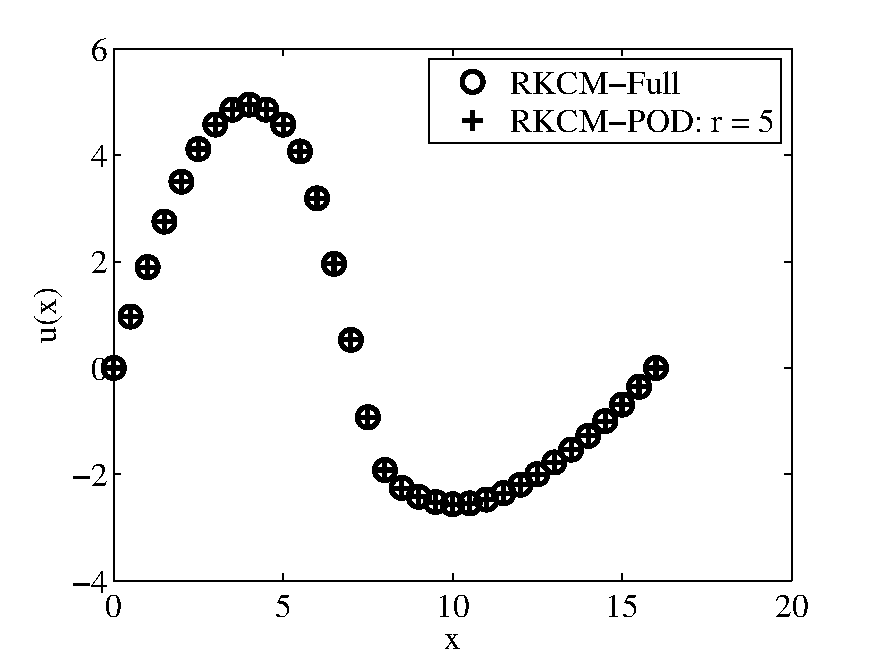
\includegraphics[width=0.5\textwidth,keepaspectratio=1,scale=1]{images/bar_T-eps-converted-to.pdf}
  \end{center}
  \caption{Comparison of the solution at the final time $T=6$ plotted over the domain, for 1D heterogeneous bar problem}
  \label{fig:7.8}
\end{figure}
%
%
\begin{table}[H]
\caption{Error $e_1$ for 1D heterogeneous bar problem}
\label{table:7.2}
\begin{center}
\begin{tabular}{| >{\centering\arraybackslash} m{2cm}| >{\centering\arraybackslash} m{2.5cm} | >{\centering\arraybackslash} m{2.5cm} |} 
\hline 
$r$ & \% DOF of full model & $e_1$  \\ %[0.5ex] % Vertical spacing
\hline \hline 
1 & 1.96\% & 5.776E+000  \\ 
\hline  
5 & 9.8\% & 3.547E-002  \\ 
\hline  
25 & 49.02\% & 3.018E-007  \\ 
\hline  
\end{tabular}
\end{center}
\end{table}
%
%




\newpage

\bibliographystyle{plain}
\bibliography{references} 

\end{document}
